\section{Replayed-Prefix On-Policy Distillation}
\label{sec:aopd}

We now turn the principle of the previous section into a concrete algorithm,
\emph{Replayed-Prefix On-Policy Distillation} (ReOPD), realized off-environment from a fixed
pool of teacher trajectories. The analysis reduces
multi-turn OPD to a single design choice: at each step, pick an effective prefix
distribution \(\rho_t\) that balances student relevance against teacher
reliability. ReOPD realizes this with two ingredients:

\begin{enumerate}[leftmargin=1.6em,itemsep=2pt,topsep=2pt]
  \item \textbf{Teacher-forced prefix, student action, teacher supervision.} For a
  supervised step \(t\), the prefix \(h_t=(O_1,A_1,\dots,O_t)\) is taken
  \emph{entirely} from a pre-collected teacher trajectory -- every earlier action
  and every observation is the teacher's recorded one. At this prefix the
  \emph{student} produces its own action, and the teacher's recorded conditional
  \(\pi_T(\cdot\mid x,h_t)\) supplies the distillation target. Sweeping \(t\) over
  the trajectory covers all positions. Because observations are always replayed,
  no environment is ever queried.
  \item \textbf{Reliability-aware step schedule.} The student is on-policy only at the
  evaluated step, on top of a teacher-forced prefix. As the position moves deeper
  into the trajectory, the replayed teacher prefix becomes a higher-shift surrogate
  for the histories the student would have reached. A per-step schedule therefore
  emphasizes early, low-shift positions and de-emphasizes late, high-shift positions
  while keeping the teacher conditional as the distillation target.
\end{enumerate}

The key point is that on-policy supervision and off-environment training coexist:
the student's step-\(t\) action makes the target relevant to the student, while the
fully teacher-forced prefix keeps the roll-in within the teacher's occupancy
(\(\mathcal P_t\approx d_T^{t}\)) and removes any environment interaction. The step schedule
then controls how these teacher-supported histories stand in for the student occupancy
\(d_{\theta_{\mathrm{old}}}^{t}\).

\paragraph{Inputs and notation.}
We are given a teacher \(\pi_T\) and a pool \(\mathcal D_T=\{(x,h)\}\) of
trajectories generated by the teacher interacting with the environment, where each
\(h\) records the full interaction history including the environment observations.
In practice this pool requires no dedicated collection: when the teacher is trained
with on-policy RL, its training rollouts are exactly such trajectories, so
\(\mathcal D_T\) is a free by-product reused for distillation.

\paragraph{Off-environment prefix construction.}
For each supervised step \(t\), the prefix \(h_t=(O_1,A_1,\dots,O_t)\) is replayed
\emph{verbatim} from the teacher trace -- all earlier actions \(A_{<t}\) and all
observations \(O_{\le t}\) are the teacher's. The student only acts at step \(t\),
where it generates its own action
\(A_t=(a_t^1,\dots,a_t^{n_t})\sim\pi_{\theta_{\mathrm{old}}}(\cdot\mid x,h_t)\)
autoregressively and is supervised, \emph{per generated token}, by the teacher's
conditional along that action, \(\pi_T(\cdot\mid x,h_t,a_t^{<j})\). Because the
supervised token contexts \(a_t^{<j}\) are the student's own samples, the evaluated
step is genuinely on-policy even though the prefix is teacher-forced, and it enters the
loss below through these on-policy contexts. No action is ever executed against the
environment and no observation is ever generated, so no environment is queried. The
roll-in is thus the teacher occupancy, \(\mathcal P_t\approx d_T^{t}\); the two-sided
shift arises because these replayed prefixes are only a surrogate for the histories the
current student would reach, a mismatch that grows with depth and that the weight below
corrects by emphasizing the shared, low-shift portion of the trajectory.

\paragraph{From the bridge to a step-decaying weight.}
The bridge weight reshapes the collected roll-in \(\mathcal P_t\approx d_T^{t}\)
toward \(\rho_t^\star\). Substituting the bridge~(\plaineqref{eq:bridge}) gives a weight that
is a power of the student-to-teacher occupancy ratio,
\[
w_t(x,h_t)
\;\propto\;
\frac{\rho_t^\star(h_t\mid x)}{\mathcal P_t(h_t\mid x)}
\;=\;
\left(\frac{d_{\theta_{\mathrm{old}}}^{t}(h_t\mid x)}{d_T^{t}(h_t\mid x)}\right)^{\gamma_t}.
\]
Because the prefix \(h_t\) is teacher-recorded and both policies act on the
\emph{same} prefix, the environment factors cancel and only the model-induced part
remains, an accumulated student-to-teacher likelihood ratio over the prefix,
\[
\widehat r_t(x,h_t)
=
\prod_{s<t}
\frac{\pi_{\theta_{\mathrm{old}}}(a_s\mid x,h_s)}{\pi_T(a_s\mid x,h_s)}.
\]
This ratio is a genuine per-history quantity -- it varies across the histories at a
fixed step \(t\) -- so the weight that realizes the bridge inside the weighted
objective~(\plaineqref{eq:weighted}) is its per-\((x,t)\)-normalized power
\begin{equation}
\label{eq:exact-weight}
w_t(x,h_t)
=
\frac{\widehat r_t(x,h_t)^{\,\gamma_t}}
{\mathbb E_{H_t\sim\mathcal P_t(\cdot\mid x)}\!\left[\widehat r_t(x,H_t)^{\,\gamma_t}\right]},
\qquad
\mathbb E_{H_t\sim\mathcal P_t}[w_t]=1,
\end{equation}
which reshapes the pooled roll-in into the effective per-step distribution
\(\rho_t=w_t\,\mathcal P_t\) exactly as the general framework prescribes, upweighting
the histories the current student is relatively more likely to have produced. Because
\(\widehat r_t\) varies within a step this normalization is non-vacuous, so
Eq.~(\plaineqref{eq:exact-weight}) is ReOPD's exact, density-ratio realization of the
bridge; it is computable from the student and teacher log-probabilities on the
recorded prefix, at the price of a high-variance per-history ratio.

Each factor compares the student's and the teacher's probability of the teacher's
own recorded action \(a_s\): since the teacher selected \(a_s\), the ratio
\(\pi_{\theta_{\mathrm{old}}}(a_s)/\pi_T(a_s)\) is typically below one, so the product
\emph{shrinks} as the prefix lengthens. Equivalently, \(\log\widehat r_t\) is a
cumulative sum that becomes more negative with depth: the further the supervised
position sits in the trajectory, the less likely the current student would have
followed the same teacher prefix, and the larger the surrogate mismatch between the
pooled prefix and the student-relevant history distribution. In other words, the
reliability weight is, to first order, a monotone \emph{step-decaying} function of the
position index.

\begin{figure}[t]
    \centering
    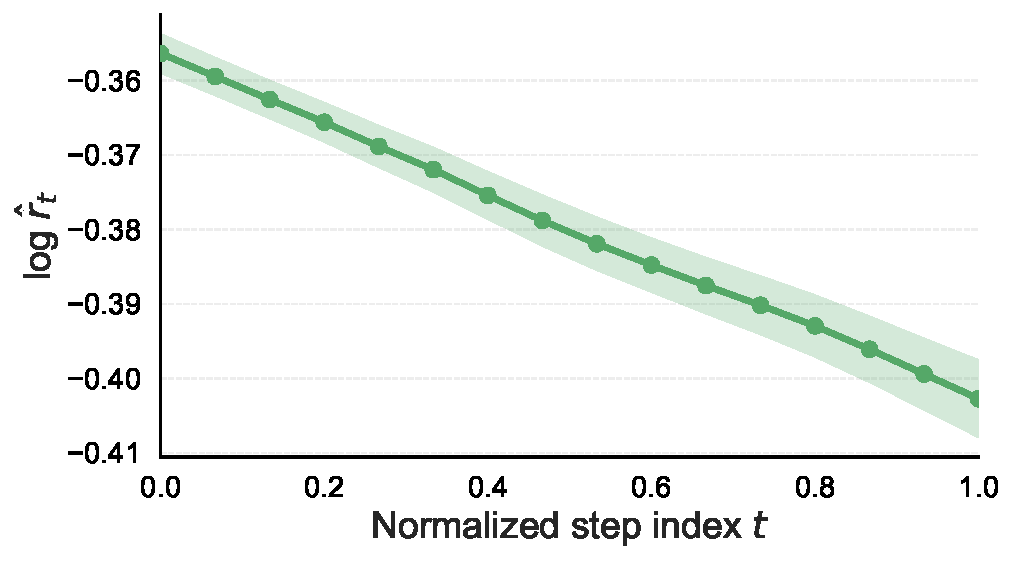
\includegraphics[width=0.6\linewidth]{figs/ratio.pdf}
    \vspace{-2mm}
  \caption[]{\textbf{Step index is a strong proxy for the likelihood-ratio weight.}
  For each supervised position we compute the per-position weight
  \(\widehat r_t=\prod_{s<t}\pi_{\theta_{\mathrm{old}}}(a_s)/\pi_T(a_s)\) -- the
  student-to-teacher likelihood ratio along the teacher prefix -- and plot it against
  the step index \(t\). The empirical weight decays with depth, because each
  factor compares the student's and teacher's probability of the teacher's own
  recorded action and is typically below one, so the product shrinks as the prefix
  lengthens. This makes step index a cheap proxy for the expensive prefix-level ratio
  and motivates replacing the explicit ratio with the one-parameter
  step-decay schedule \(\omega(t)=\kappa^{t}\) introduced below.}
  \label{fig:weight_decay}
  \vspace{-3mm}
\end{figure}

This holds empirically, not just to first order: measured directly along teacher
prefixes, \(\widehat r_t\) is tightly organized by step index
(Figure~\ref{fig:weight_decay}), so depth explains most of its variation and justifies
the design choice we make next -- replacing the expensive, high-variance per-prefix
ratio with a stable depth-based proxy.

Concretely, the surrogate keeps the monotone-decreasing \emph{shape} of the exact
weight~(\plaineqref{eq:exact-weight}) while dropping the noisy per-history factor
\(\widehat r_t\); both the shape and the right steepness follow from the exact weight
itself. Writing the average per-step teacher--student gap along the prefix as
\[
\bar c(x)
=
\mathbb E_{a_s\sim\pi_T}\!\left[
\log\frac{\pi_T(a_s\mid x,h_s)}{\pi_{\theta_{\mathrm{old}}}(a_s\mid x,h_s)}
\right]
\;\ge\;0
\qquad(\text{an average per-step } D_{\mathrm{KL}}(\pi_T\,\|\,\pi_{\theta_{\mathrm{old}}})),
\]
we have \(\log\widehat r_t\approx-(t-1)\,\bar c\), so the exact weight's depth profile
is geometric:
\begin{equation}
\label{eq:kappa-map}
\widehat r_t^{\,\gamma_t}\;\approx\;\kappa^{\,t}\ \text{(up to a constant)},
\qquad
\kappa=\exp\!\left(-\gamma_t\,\bar c\right)\in(0,1].
\end{equation}
This is the bridge-to-schedule map: the decay \emph{base} \(\kappa\) is not a free
prefactor but is pinned by the bridge exponent \(\gamma_t\) (how far \(\rho_t\) is
pushed toward the student occupancy) and the per-step gap \(\bar c\) (how fast the
teacher pool diverges from the student with depth), and shrinks -- steeper decay --
when either grows. Collapsing the profile to a single base \(\kappa\) treats the
per-step gap as approximately stationary across positions; when it instead grows with
depth, \(\kappa^{t}\) is a first-order (geometric-mean) approximation to the true
accumulated ratio, which Figure~\ref{fig:weight_decay} shows already tracks the measured
decay well. ReOPD therefore uses the one-parameter schedule
\[
\omega(t;\kappa)=\kappa^{\,t}
\qquad(\text{or any monotone decreasing schedule}),
\]
with \(\kappa\in(0,1]\) the single steepness knob; the overall scale cancels under
normalization, so -- unlike a raw power law -- there is no separate prefactor, and in
particular no scale symbol to collide with the bridge exponent \(\gamma_t\). This is the surrogate's reliability weight,
\(w_t=\omega(t;\kappa)=\kappa^{\,t}\). Because it depends only on the position index it
is constant across the histories at a fixed \(t\), so it is normalized \emph{over the
horizon} -- across positions, in proportion to \(\kappa^{\,t}\) -- rather than
per-\((x,t)\); a per-\((x,t)\) normalization would send a step-constant weight to
\(w_t\!\equiv\!1\) and erase the decay. This makes the trade-off between the two forms
explicit: both feed the same weighted objective~(\plaineqref{eq:weighted}) through the
effective distribution \(\rho_t\propto w_t\,\mathcal P_t\), but the exact
weight~(\plaineqref{eq:exact-weight}) varies \emph{within} each step (per-\((x,t)\)
normalization -- a genuine density ratio that reshapes histories at a fixed \(t\)),
whereas the step-decay surrogate varies \emph{across} steps (horizon normalization --
constant within a step) and so reallocates mass toward the early, low-shift positions.
They differ only in the axis along which \(w_t\) carries the reliability signal. The surrogate trades exactness for a single interpretable
knob: \(\kappa\!=\!1\) recovers uniform weighting across positions (no decay), and
smaller \(\kappa\) concentrates supervision on the early, more reliable steps. Both
forms point the same way, since \(\widehat r_t\) decays with depth; the surrogate is
the default we sweep in Section~\ref{sec:experiments}, realized by sampling positions
in proportion to it (equivalently, as a loss weight), as detailed next. More generally the weight can be
made data-dependent -- e.g.\ derived from the student's own sampling probabilities at
the evaluated step.

\paragraph{Weighted distillation objective.}
At each supervised step the student samples its own action
\(A_t=(a_t^1,\dots,a_t^{n_t})\sim\pi_{\theta_{\mathrm{old}}}(\cdot\mid x,H_t)\) and is
distilled against the teacher \emph{along that action}: the per-step loss is the
token-level KL accumulated over the student-sampled action tokens,
\[
\ell\big(\pi_\theta,\pi_T;x,H_t,A_t\big)
=
\sum_{j=1}^{n_t}
D_{\mathrm{KL}}\!\Big(
\pi_\theta(\cdot\mid x,H_t,a_t^{<j})
\,\big\|\,
\pi_T(\cdot\mid x,H_t,a_t^{<j})
\Big),
\]
whose conditioning contexts \(a_t^{<j}\) are on-policy, so the loss depends on the
student's action. The student then minimizes the reweighted step-wise objective
\[
\mathcal L(\theta)
=
\mathbb E_{x\sim\mathcal D}
\left[
\sum_{t=1}^{T}\alpha_t\,
\mathbb E_{H_t\sim\mathcal P_t(\cdot\mid x)}
\;
\mathbb E_{A_t\sim\pi_{\theta_{\mathrm{old}}}(\cdot\mid x,H_t)}
\Big[
w_t\,
\ell\big(\pi_\theta,\pi_T;x,H_t,A_t\big)
\Big]
\right].
\]
Here \(\alpha_t\) is the uniform base of Section~\ref{sec:formulation} and the
reliability signal is carried entirely by \(w_t\): the exact weight sets \(w_t\) by
Eq.~(\plaineqref{eq:exact-weight}) (per-\((x,t)\)-normalized), while the step-decay
surrogate sets \(w_t=\omega(t;\kappa)=\kappa^{t}\) (horizon-normalized). The effective
per-position mass is then \(\alpha_t\,w_t\,\mathcal P_t\propto w_t\,\mathcal P_t\), which
the next paragraph draws from directly.
After optimization the student is refreshed, \(\theta_{\mathrm{old}}\leftarrow\theta\),
and the next iteration re-evaluates the student's steps against the same teacher
prefixes, so supervision tracks the moving student while staying anchored to the
teacher pool.

\paragraph{From the objective to sampling.}
The design target is a \emph{distribution}, not a weight: objective~(\plaineqref{eq:rho-obj})
is the plain (unweighted) loss in expectation under \(\rho_t^\star\). Any unbiased
Monte-Carlo estimate of that expectation is a valid implementation, and there are two
natural ones.
\emph{(i) Sampling (direct).} Estimate~(\plaineqref{eq:rho-obj}) by drawing histories
from \(\rho_t^\star\) and averaging the \emph{unweighted} loss. Since the pool only
provides samples from \(\mathcal P_t\), we draw positions with
\(p_t\propto w_t\,\mathcal P_t=\rho_t^\star\) -- i.e.\ resample the pooled positions in
proportion to the step-decay schedule -- and apply the loss with no reweighting. This
is the direct estimator of~(\plaineqref{eq:rho-obj}): the schedule appears only in
\emph{which} positions are trained, matching how the offline pool is streamed and
touching only a subset of positions per step.
\emph{(ii) Weighting (importance).} Keep the pooled samples from \(\mathcal P_t\) and
instead multiply the loss by \(w_t\). The importance identity
\(\mathbb E_{H_t\sim\mathcal P_t}[w_t\,\ell]=\mathbb E_{H_t\sim\rho_t^\star}[\ell]\)
makes this the importance-weighted estimator of the \emph{same} expectation, at a
compute cost proportional to enumerating every position.
Sampling is therefore not an approximation of weighting: both are unbiased estimators
of the single distributional objective~(\plaineqref{eq:rho-obj}), with sampling the more
direct one. We use \emph{sampling} in all experiments and treat weighting as an
equivalent alternative.

\paragraph{Setting the decay.}
The only free knob is the steepness \(\kappa\). The map~(\plaineqref{eq:kappa-map})
makes it measurable: \(\kappa\approx\exp(-\gamma_t\bar c)\) is read off from the
per-step teacher--student gap \(\bar c\), an average
\(D_{\mathrm{KL}}(\pi_T\|\pi_{\theta_{\mathrm{old}}})\) estimated directly on the pool.
The weight always decreases with depth, so early, low-shift steps receive the most
mass and \(\kappa\) only sets how fast it falls off: \(\kappa\!=\!1\) is uniform
(OPD-like) and smaller \(\kappa\) concentrates supervision on the early steps. The two
regimes read off through \(\bar c\) -- a small gap gives \(\kappa\!\approx\!1\) and
gentle decay, a large gap (e.g.\ the wide teacher--student math setting) gives small
\(\kappa\) and steep decay -- and steepness is set empirically in
Section~\ref{sec:experiments}, entering only through the sampling probability
\(p_t\propto w_t\) (equivalently, a weight \(w_t\)).

\begin{algorithm}[t]
\caption{Replayed-Prefix On-Policy Distillation (ReOPD)}
\label{alg:aopd}
\begin{algorithmic}[1]
\Require teacher pool \(\mathcal D_T\), teacher \(\pi_T\), student \(\pi_\theta\),
step-decay schedule \(\omega(t;\kappa)=\kappa^{t}\)
\State initialize \(\theta_{\mathrm{old}}\leftarrow\theta\)
\For{each OPD iteration}
  \State assemble candidate positions \(\{(x,h_t)\}\) from pooled trajectories \Comment{prefix \(h_t\): teacher actions \(A_{<t}\), teacher observations \(O_{\le t}\)}
  \State draw positions with \(p_t\propto\omega(t;\kappa)\) \Comment{early, low-shift steps sampled more often}
  \For{each sampled position \((x,h_t)\)}
    \State student generates its action \(A_t=(a_t^1,\dots,a_t^{n_t})\sim\pi_{\theta_{\mathrm{old}}}(\cdot\mid x,h_t)\) \Comment{token contexts on-policy; no environment call}
    \State accumulate \(\sum_{j=1}^{n_t} D_{\mathrm{KL}}\!\big(\pi_\theta(\cdot\mid x,h_t,a_t^{<j})\,\|\,\pi_T(\cdot\mid x,h_t,a_t^{<j})\big)\) \Comment{per-token KL along the student's action \(A_t\)}
  \EndFor
  \State update \(\theta\) on the accumulated loss; \(\theta_{\mathrm{old}}\leftarrow\theta\)
\EndFor
\State \Return \(\pi_\theta\)
\end{algorithmic}
\end{algorithm}

\paragraph{Why this is more than ``make it on-policy''.}
Standard OPD pushes prefixes toward the student by re-rolling through a live
environment; ReOPD instead replays a teacher-forced prefix and corrects with a
reliability-aware step-decay schedule, achieving student relevance off-environment. The
principle is reliability-aware prefix distribution design, which we implement by
sampling prefixes along that schedule.

\paragraph{Relation to RL and distillation.}
ReOPD sits between reinforcement learning and distillation, and the bridge parameter
\(\gamma_t\) is precisely the slider between them. Like on-policy RL, the student
acts at the supervised step and is trained on its own actions, so the signal is
relevant to what the student will do; like distillation, the supervision is the
teacher's full per-step conditional \(\pi_T(\cdot\mid x,h_t)\) rather than a scalar
return. This is the sense in which on-policy distillation provides a \emph{dense}
improvement signal where RL provides a sparse one~\citep{thinkingmachines2025onpolicy}:
RL conveys a few bits per episode, whereas matching a distribution supervises every
token. In our occupancy language, \(\gamma_t\!\to\!1\) places the effective prefix
distribution at the student occupancy \(d_{\theta_{\mathrm{old}}}^{t}\) -- the regime
on-policy methods target -- while \(\gamma_t\!\to\!0\) places it at the teacher
occupancy \(d_T^{t}\) -- ordinary teacher-forced distillation -- and intermediate
values interpolate.

This should not be mistaken for off-policy or reward-weighted RL. We do not estimate
returns or advantages, apply no importance-sampling correction to a value function,
and never optimize a scalar reward; the target is a fixed teacher distribution and
the weight \(w_t\) encodes the reliability and student-relevance of the replayed
prefix, not a policy-gradient ratio. Nor do we require environment interaction: the
``on-policy'' part is the
student's action at a single step on a replayed prefix, not a fresh rollout. ReOPD is
thus best read as distillation with an on-policy supervised step and a
reliability-aware prefix distribution -- inheriting the relevance of RL-style
on-policy data and the density of distillation, while avoiding both the sparsity of
reward and the cost of online rollouts.